\section{阻尼Newton法}
\label{sec:newton-damped}

上一节的定理只管解附近。接下来要弄清：Hessian仍然正定，但当前点离解很远，模型的底不可信，怎样在不改变方向的前提下保证目标确实下降，又不损失解附近的快速收敛？

\paragraph{完整Newton步的麻烦}
回到目标~\eqref{eq:newton-running-objective}，从$\bm{x}^{(0)}=(-1,\tfrac65)$出发。此处$u=\tfrac15$，Hessian的行列式是$2(1-4u)=0.4$，正定但接近奇异。由式~\eqref{eq:newton-running-direction}，
\[
 d_1=\frac{2}{0.2}=10,\qquad d_2=-\frac15-2\cdot10=-20.2.
\]
走满一步到达$(9,-19)$，目标从$2.04$升到$10032$。

Newton方向在这里是下降方向，毛病出在走得太远。按式~\eqref{eq:newton-running-direction}继续走完整步，迭代点在$(9,-19)$、$(8.98,80.6)$、$(1.01,-62.5)$之间大幅跳动，几步之后才落回解附近，见图~\ref{fig:newton-damped-path}(a)。这条路径能回来，靠的是上一节提到的此目标的特殊结构。一般目标没有这种运气，式~\eqref{eq:newton-cubic-map}的发散就是例子。

\paragraph{主要思想}
Newton方向是模型认为最好的方向，模型的问题主要在于它在远处高估了自己。一个自然的补救是保留方向，但只走其中的一段，走多少由原目标来核验：
\begin{equation}
 \bm{x}^{(t+1)}=\bm{x}^{(t)}+\alpha^{(t)}\bm{d}^{(t)},\qquad 0<\alpha^{(t)}\leq1.
 \label{eq:newton-damped-update}
\end{equation}
这称为\term{阻尼Newton法}（damped Newton method）。方向仍由方程~\eqref{eq:newton-equation}确定，改变的只是这一步信模型信到什么程度。

核验用第~\ref{chap:smooth-foundations}章的Armijo条件。给定$c\in(0,\tfrac12)$，要求实际下降至少达到一阶预测的$c$倍：
\begin{equation}
 f(\bm{x}^{(t)}+\alpha\bm{d}^{(t)})\leq f(\bm{x}^{(t)})+c\,\alpha\,(\bm{g}^{(t)})^\top\bm{d}^{(t)}.
 \label{eq:newton-armijo}
\end{equation}
回溯的做法是先试$\alpha=1$，不满足就乘以$\beta\in(0,1)$，直到满足为止。上限取$1$、并且先试$1$，理由在本节后面说明。

方向导数$(\bm{g}^{(t)})^\top\bm{d}^{(t)}$在这里有专门的意义。记
\begin{equation}
 (\omega^{(t)})^2=-(\bm{g}^{(t)})^\top\bm{d}^{(t)}=(\bm{g}^{(t)})^\top(\bm{H}^{(t)})^{-1}\bm{g}^{(t)}.
 \label{eq:newton-decrement}
\end{equation}
$\omega^{(t)}$称为\term{Newton减量}（Newton decrement）。把$\bm{d}^{(t)}$代入模型，再用$\bm{H}^{(t)}\bm{d}^{(t)}=-\bm{g}^{(t)}$，得到模型的预测下降量
\[
 m^{(t)}(\bm{0})-m^{(t)}(\bm{d}^{(t)})=\frac12(\omega^{(t)})^2.
\]
所以$\tfrac12(\omega^{(t)})^2$是模型对“还能下降多少”的估计，可以作为停止标准。它和Newton方向一样不受坐标伸缩影响，梯度范数则没有这种性质。

\paragraph{正定性为回溯提供了什么}
回溯要能结束，当前方向必须是下降方向。由式~\eqref{eq:newton-descent}，$\bm{H}^{(t)}\succ\bm{0}$时$(\omega^{(t)})^2>0$。把目标限制在这个方向上，记一元函数$\varphi(\alpha)$为沿方向走$\alpha$时的目标值，它在$0$处的导数是$-(\omega^{(t)})^2<0$，于是
\[
 \varphi(\alpha)=\varphi(0)-\alpha(\omega^{(t)})^2+o(\alpha).
\]
由于$c<1$，当$\alpha$足够小时，式~\eqref{eq:newton-armijo}成立，回溯在有限次内结束。

如果$\bm{H}^{(t)}$不定，这个保证就没有了。第~\ref{sec:newton-basic}节的点$(0,\tfrac12)$处方向导数为$\tfrac12>0$，式~\eqref{eq:newton-armijo}的右端随$\alpha$增大而升高，而左端在小$\alpha$上升得比右端更快，因为$c<1$。无论$\alpha$多小都不满足，回溯永远停不下来。阻尼只能调整走多远，不能把上坡的方向变成下坡。

\paragraph{计算过程}
仍用目标~\eqref{eq:newton-running-objective}，从上面的坏起点$(-1,\tfrac65)$出发。

\needspace{6\baselineskip}
\paragraph{变量}
\begin{itemize}
 \item $\bm{x},\bm{g},\bm{H},\bm{d}$：与Newton法相同，分别是当前点、梯度、Hessian和Newton方向。
 \item $\omega^2$：Newton减量的平方，同时是方向导数的相反数。
 \item $\alpha$：当前试探步长，每轮从$1$开始。
 \item $c,\beta$：Armijo参数和回溯因子，全程固定。
 \item $\varepsilon$：停止容差，判断$\tfrac12\omega^2\leq\varepsilon$。
\end{itemize}

\paragraph{初始化}
选定$\bm{x}^{(0)}$，$c\in(0,\tfrac12)$，$\beta\in(0,1)$，$\varepsilon>0$。例中取下面的数据：
\[
 \bm{x}^{(0)}=\bigl(-1,\tfrac65\bigr),\qquad c=0.1,\qquad \beta=0.5,\qquad \varepsilon=10^{-10}.
\]

\needspace{6\baselineskip}
\paragraph{每轮更新}
在第$t$轮：
\begin{enumerate}
 \item \textbf{求Newton方向。}计算$\bm{g}^{(t)}$、$\bm{H}^{(t)}$，用Cholesky分解解方程~\eqref{eq:newton-equation}。

 例中第一轮
 \[
  \bm{g}^{(0)}=\begin{bmatrix}-1.2\\0.4\end{bmatrix},\qquad
  \bm{H}^{(0)}=\begin{bmatrix}8.2&4\\4&2\end{bmatrix},\qquad
  \bm{d}^{(0)}=\begin{bmatrix}10\\-20.2\end{bmatrix}.
 \]

 \item \textbf{检查停止。}按式~\eqref{eq:newton-decrement}计算$\omega^2$。若$\tfrac12\omega^2\leq\varepsilon$，输出$\bm{x}^{(t)}$并结束。

 例中第一轮
 \[
  (\omega^{(0)})^2=12+8.08=20.08.
 \]

 \item \textbf{回溯。}令$\alpha=1$。当式~\eqref{eq:newton-armijo}不成立时，令$\alpha\leftarrow\beta\alpha$。

 例中第一轮的右端是$2.04-2.008\alpha$，试探结果如下：
 \[
  \begin{array}{ccccc}
   \alpha&1&1/2&1/4&1/8\\
   f(\bm{x}^{(0)}+\alpha\bm{d}^{(0)})&10032&624.5&37.34&2.206\\
   \text{右端}&0.032&1.036&1.538&1.789
  \end{array}
 \]
 四次都被拒绝。下一次试探$\alpha=\tfrac1{16}$，新点是$(-0.375,-0.0625)$，目标值$0.9866$，右端$1.9145$，条件满足，接受。

 \item \textbf{更新。}按式~\eqref{eq:newton-damped-update}走到下一点，令$t\leftarrow t+1$。

 例中第一轮到达$\bm{x}^{(1)}=(-0.375,-0.0625)$。

 第二轮$u=-0.203125$，由式~\eqref{eq:newton-running-derivatives}和式~\eqref{eq:newton-running-direction}，
 \[
  \bm{g}^{(1)}=\begin{bmatrix}-1.6797\\-0.4063\end{bmatrix},\qquad
  \bm{d}^{(1)}=\begin{bmatrix}0.7586\\-0.3658\end{bmatrix},\qquad
  (\omega^{(1)})^2=1.1256.
 \]
 试探$\alpha=1$，新点的目标值是$0.5212$，右端是$0.9866-0.1126=0.8740$，第一次试探即被接受。
\end{enumerate}

图~\ref{fig:newton-backtrack}是第一轮回溯的情形。表~\ref{tab:newton-damped-run}列出各轮结果。第$1$轮以后每次都是$\alpha=1$第一次就被接受。第$7$轮$\tfrac12\omega^2$已低于容差，迭代结束，最终得到$\bm{x}^{(7)}\approx(1,1)$，目标值约$7.6\times10^{-15}$。

\begin{BookInlineFigure}
  \centering
  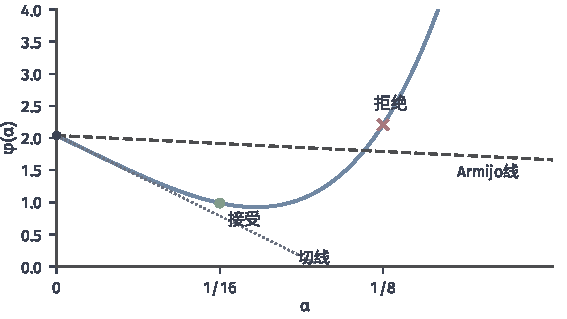
\includegraphics[width=96mm]{figures/05-optimization/02-smooth-optimization/matplotlib/newton-backtrack/figure.pdf}
  \caption{第一轮回溯沿方向的一元函数$\varphi(\alpha)=f(\bm{x}^{(0)}+\alpha\bm{d}^{(0)})$（蓝）。灰色点线是$\alpha=0$处的切线，深灰色虚线是Armijo线$\varphi(0)+c\alpha\varphi'(0)$，曲线在Armijo线下方的步长才可接受。$\alpha=\tfrac18$处（红叉）目标在线上方，被拒绝；$\alpha=\tfrac1{16}$处（绿点）被接受。$\alpha=1,\tfrac12,\tfrac14$在图外，目标值更高。}
  \label{fig:newton-backtrack}
\end{BookInlineFigure}

\begin{BookInlineTable}
  \centering
  \begin{tabular}{@{}ccccc@{}}
    \toprule
    $t$ & $\bm{x}^{(t)}$ & $f$ & $(\omega^{(t)})^2$ & $\alpha^{(t)}$ \\
    \midrule
    $0$ & $(-1,1.2)$ & $2.04$ & $20.08$ & $1/16$ \\
    $1$ & $(-0.375,-0.0625)$ & $0.9866$ & $1.1256$ & $1$ \\
    $2$ & $(0.3836,-0.4283)$ & $0.5212$ & $0.7775$ & $1$ \\
    $3$ & $(0.5703,0.2904)$ & $0.09354$ & $0.1645$ & $1$ \\
    $4$ & $(0.9474,0.7554)$ & $0.02161$ & $0.04223$ & $1$ \\
    $5$ & $(0.9809,0.9611)$ & $1.83\mathrm{e}{-4}$ & $3.64\mathrm{e}{-4}$ & $1$ \\
    $6$ & $(0.99992,0.99947)$ & $1.33\mathrm{e}{-7}$ & $2.67\mathrm{e}{-7}$ & $1$ \\
    $7$ & $(1.0000,1.0000)$ & $7.6\mathrm{e}{-15}$ & $1.5\mathrm{e}{-14}$ & 停止 \\
    \bottomrule
  \end{tabular}
  \caption{阻尼Newton法从$(-1,\tfrac65)$出发的迭代，$c=0.1$，$\beta=0.5$。只有第一轮的方向需要缩短，其余各轮都接受完整步。}
  \label{tab:newton-damped-run}
\end{BookInlineTable}

\begin{BookInlineFigure}
  \centering
  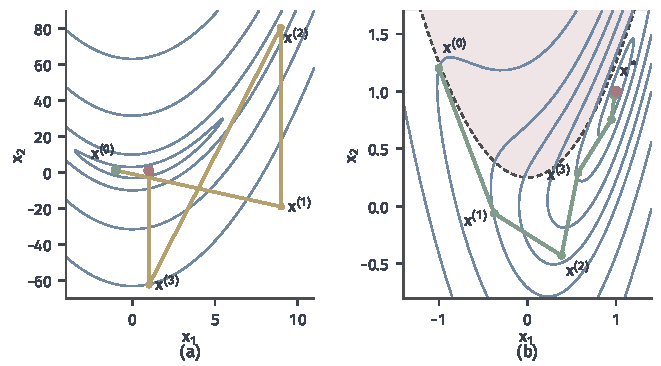
\includegraphics[width=112mm]{figures/05-optimization/02-smooth-optimization/matplotlib/newton-damped-path/figure.pdf}
  \caption{从$(-1,\tfrac65)$出发的两条路径，蓝线是等高线，红点是解。(a)完整Newton步（黄）在大范围内来回跳动，纵轴范围约$160$。(b)阻尼Newton法（绿）第一步只走$\tfrac1{16}$，随后沿山谷收敛，红色浅底是Hessian不定的区域。}
  \label{fig:newton-damped-path}
\end{BookInlineFigure}

图~\ref{fig:newton-damped-history}把目标值和步长画成曲线。完整Newton步的目标值先冲到$10^4$的量级，阻尼方法则严格逐步下降。值得注意的是，完整步的路径从第$4$轮起目标值反而更低，因为它恰好跳到了解附近；阻尼保证的是每一步可靠，并不保证每条路径的步数都最少。

\begin{BookInlineFigure}
  \centering
  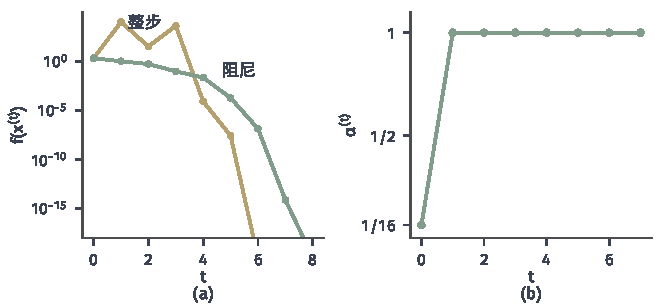
\includegraphics[width=112mm]{figures/05-optimization/02-smooth-optimization/matplotlib/newton-damped-history/figure.pdf}
  \caption{图~\ref{fig:newton-damped-path}两条路径的数值。(a)目标值的半对数曲线，绿线为阻尼Newton法，黄线为完整Newton步。(b)阻尼Newton法各轮接受的步长，第一轮之后都是$1$。}
  \label{fig:newton-damped-history}
\end{BookInlineFigure}

\paragraph{强凸目标上的全局收敛}
现在把“回溯总能带来足够下降”写成定理。定理需要曲率的上下界，用来保证方向既不太长也不太偏。假设对全空间成立是为了证明简洁；真正用到的只是初始下水平集附近的界，这时要额外说明所有试探点留在该区域内。

\begin{theorem}[阻尼Newton法的全局线性收敛]
\label{thm:newton-damped-global}
设$f$二阶连续可微，且对所有$\bm{x}$，$\mu\bm{I}\preceq\nabla^2f(\bm{x})\preceq L\bm{I}$，其中$0<\mu\leq L$，记$\kappa=L/\mu$。取$c\in(0,\tfrac12)$，$\beta\in(0,1)$。则回溯总在有限次内结束，接受的步长满足$\alpha^{(t)}\geq\beta/\kappa$，并且
\begin{equation}
 f(\bm{x}^{(t+1)})-f^\star\leq\Bigl(1-\frac{2c\beta}{\kappa^2}\Bigr)\bigl(f(\bm{x}^{(t)})-f^\star\bigr).
 \label{eq:newton-damped-linear}
\end{equation}
\end{theorem}

\begin{proof}
省略上标。第一步估计沿方向的上界。曲率上界$L$给出
\[
 f(\bm{x}+\alpha\bm{d})\leq f(\bm{x})+\alpha\bm{g}^\top\bm{d}+\frac L2\alpha^2\lVert\bm{d}\rVert_2^2.
\]
由式~\eqref{eq:newton-decrement}，$\bm{g}^\top\bm{d}=-\omega^2$。又由$\bm{H}\succeq\mu\bm{I}$，
\[
 \omega^2=\bm{d}^\top\bm{H}\bm{d}\geq\mu\lVert\bm{d}\rVert_2^2.
\]
代入上式，
\[
 f(\bm{x}+\alpha\bm{d})\leq f(\bm{x})-\alpha\omega^2+\frac\kappa2\alpha^2\omega^2.
\]

第二步确定可接受的步长范围。与式~\eqref{eq:newton-armijo}比较，只要$-1+\tfrac\kappa2\alpha\leq-c$，也就是$\alpha\leq2(1-c)/\kappa$，Armijo条件就成立。

第三步给出步长下界。若$\alpha=1$被接受，则$\alpha=1\geq\beta/\kappa$。否则上一个试探值$\alpha/\beta$被拒绝，必有$\alpha/\beta>2(1-c)/\kappa$。由$c<\tfrac12$得$2(1-c)>1$，所以$\alpha>\beta/\kappa$。

第四步估计下降量。由式~\eqref{eq:newton-armijo}和步长下界，
\[
 f(\bm{x})-f(\bm{x}^{(t+1)})\geq c\alpha\omega^2\geq\frac{c\beta}\kappa\omega^2.
\]
由$\bm{H}^{-1}\succeq L^{-1}\bm{I}$，有$\omega^2\geq\lVert\bm{g}\rVert_2^2/L$。

第五步用梯度控制目标差。强凸性给出，对任意$\bm{y}$，
\[
 f(\bm{y})\geq f(\bm{x})+\bm{g}^\top(\bm{y}-\bm{x})+\frac\mu2\lVert\bm{y}-\bm{x}\rVert_2^2\geq f(\bm{x})-\frac{\lVert\bm{g}\rVert_2^2}{2\mu},
\]
其中第二个不等号是对$\bm{y}$取右端的最小值。令$\bm{y}=\bm{x}^\star$，得$\lVert\bm{g}\rVert_2^2\geq2\mu(f(\bm{x})-f^\star)$。

综合第四、第五步，
\[
 f(\bm{x})-f(\bm{x}^{(t+1)})\geq\frac{c\beta}{\kappa L}\cdot2\mu\bigl(f(\bm{x})-f^\star\bigr)=\frac{2c\beta}{\kappa^2}\bigl(f(\bm{x})-f^\star\bigr).
\]
两边减$f^\star$后整理，即得式~\eqref{eq:newton-damped-linear}。
\end{proof}

这个速率含$\kappa^2$，远比实际表现差，而且算法本身不受坐标伸缩的影响，界却依赖坐标下的$\mu,L$。定理的作用不在于预测步数，而在于保证从任何起点出发目标都稳定下降，梯度趋于零。要得到不依赖坐标的步数界，需要对三阶导数作更细致的假设，证明篇幅较长，读者可查阅\scite{math-boyd2004convex}。

\paragraph{完整步何时恢复}
全局定理保证迭代进入解的附近，但如果进入后步长仍小于$1$，局部二次收敛就得不到。表~\ref{tab:newton-damped-run}显示步长很快回到$1$，下面的定理说明这不是偶然。

\begin{theorem}[完整步的接受与二次收敛]
\label{thm:newton-unit-step}
在定理~\ref{thm:newton-damped-global}的条件下，再设$\nabla^2f$是$M$-Lipschitz的，记
\begin{equation}
 \tau=\min\bigl\{1,\,3(1-2c)\bigr\}\frac{\mu^2}{M}.
 \label{eq:newton-unit-threshold}
\end{equation}
若$\lVert\bm{g}^{(t)}\rVert_2\leq\tau$，则$\alpha=1$通过Armijo检验，且
\begin{equation}
 \lVert\bm{g}^{(t+1)}\rVert_2\leq\frac{M}{2\mu^2}\lVert\bm{g}^{(t)}\rVert_2^2\leq\frac12\lVert\bm{g}^{(t)}\rVert_2.
 \label{eq:newton-gradient-quadratic}
\end{equation}
因此一旦某轮梯度范数不超过$\tau$，此后每轮都接受完整步，梯度范数二次收敛到零。
\end{theorem}

\begin{proof}
省略上标。令$h(s)=f(\bm{x}+s\bm{d})$。先用Taylor公式的积分余项写出
\[
 h(1)=h(0)+h'(0)+\int_0^1(1-s)h''(s)\,\mathrm{d}s.
\]
这里$h'(0)=-\omega^2$。由Hessian的Lipschitz条件，
\[
 h''(s)=\bm{d}^\top\nabla^2f(\bm{x}+s\bm{d})\bm{d}\leq\omega^2+Ms\lVert\bm{d}\rVert_2^3.
\]
代入积分，得到
\[
 f(\bm{x}+\bm{d})\leq f(\bm{x})-\frac12\omega^2+\frac M6\lVert\bm{d}\rVert_2^3.
\]

要通过Armijo检验，只需
\[
 \frac M6\lVert\bm{d}\rVert_2^3\leq\Bigl(\frac12-c\Bigr)\omega^2.
\]
由$\lVert\bm{d}\rVert_2^2\leq\omega^2/\mu$，只需$\lVert\bm{d}\rVert_2\leq3(1-2c)\mu/M$。而$\lVert\bm{d}\rVert_2\leq\lVert\bm{g}\rVert_2/\mu$，所以条件$\lVert\bm{g}\rVert_2\leq3(1-2c)\mu^2/M$足够。

再看新点的梯度。沿线段积分并用$\bm{g}+\bm{H}\bm{d}=\bm{0}$，得到
\[
 \nabla f(\bm{x}+\bm{d})=\int_0^1\bigl(\nabla^2f(\bm{x}+s\bm{d})-\bm{H}\bigr)\bm{d}\,\mathrm{d}s.
\]
被积项范数不超过$Ms\lVert\bm{d}\rVert_2^2$，积分后得到
\[
 \lVert\nabla f(\bm{x}+\bm{d})\rVert_2\leq\frac M2\lVert\bm{d}\rVert_2^2\leq\frac{M}{2\mu^2}\lVert\bm{g}\rVert_2^2.
\]
再由$\lVert\bm{g}\rVert_2\leq\mu^2/M$，得到式~\eqref{eq:newton-gradient-quadratic}的第二个不等号。新点的梯度范数仍不超过$\tau$，归纳即得结论。
\end{proof}

两个定理合起来刻画了整段迭代。在定理~\ref{thm:newton-damped-global}的保证下，目标差趋于零；由$\lVert\bm{g}\rVert_2^2\leq2L(f(\bm{x})-f^\star)$，梯度范数在有限步内降到$\tau$以下；从此进入完整步阶段，速度由定理~\ref{thm:newton-unit-step}给出。线搜索负责把迭代带到解附近，然后自动退出。

\paragraph{为什么先试$\alpha=1$，为什么$c<\tfrac12$}
先试$\alpha=1$不是习惯，而是快速收敛的必要条件。若永远用固定的$\alpha<1$，在解附近目标接近二次，误差满足$\bm{e}^{(t+1)}\approx(1-\alpha)\bm{e}^{(t)}$，收敛退化为线性。图~\ref{fig:newton-unit-step}(a)显示，$\alpha=0.9$和$\alpha=0.5$都只有直线下降，$\alpha=0.5$时误差每步减半。

$c<\tfrac12$同样与完整步有关。在二次目标上，沿Newton方向有精确的下降量
\[
 h(\alpha)-h(0)=-\alpha\omega^2+\frac12\alpha^2\omega^2.
\]
取$\alpha=1$得$-\tfrac12\omega^2$，Armijo的右端是$-c\omega^2$。所以$c\leq\tfrac12$时完整步可接受，$c>\tfrac12$时连精确的模型极小点都被拒绝，如图~\ref{fig:newton-unit-step}(b)所示。

\begin{BookInlineFigure}
  \centering
  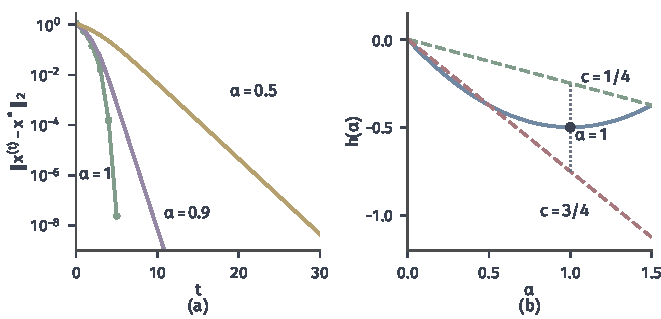
\includegraphics[width=112mm]{figures/05-optimization/02-smooth-optimization/matplotlib/newton-unit-step/figure.pdf}
  \caption{完整步的作用。(a)目标~\eqref{eq:newton-running-objective}上从$(\tfrac12,0)$出发、使用固定步长的距离误差：绿线$\alpha=1$，紫线$\alpha=0.9$，黄线$\alpha=0.5$。(b)二次目标沿Newton方向的变化量$h(\alpha)$（蓝，取$\omega^2=1$），绿色和红色虚线分别是$c=\tfrac14$和$c=\tfrac34$的Armijo线。$\alpha=1$处的黑点在绿线下方、红线上方，所以前者接受、后者拒绝。}
  \label{fig:newton-unit-step}
\end{BookInlineFigure}

回溯只需要函数值，每次试探一次函数计算。Newton方向的尺度已经带上了曲率信息，试探通常一两次就结束，所以这里用Armijo条件就够了。第~\ref{chap:smooth-foundations}章中要求方向导数的线搜索条件，主要用在方向尺度不明确或曲率更新需要额外保证的方法上。
